%%%%%%%%%%%%%%%%%%%%%%% file template.tex %%%%%%%%%%%%%%%%%%%%%%%%%
%
% This is a template file for Web of Conferences Journal
%
% Copy it to a new file with a new name and use it as the basis
% for your article
%
%%%%%%%%%%%%%%%%%%%%%%%%%% EDP Science %%%%%%%%%%%%%%%%%%%%%%%%%%%%
%
%%%\documentclass[option]{webofc}
%%% "twocolumn" for typesetting an article in two columns format (default one column)
%
\documentclass{webofc}
\usepackage[varg]{txfonts}   % Web of Conferences font
%
% Put here some packages required or/and some personal commands

\usepackage{xspace}


\newcommand{\pd}{protoDUNE\xspace}
\newcommand{\filesize}{8\,GB\xspace}


%
%
\begin{document}
%
\title{The \pd-SP prompt processing system and its application in Data Quality Monitoring}
%
%%%\subtitle{Do you have a subtitle?\\ If so, write it here}
\author{\firstname{First author} \lastname{First author}\inst{1,3}\fnsep\thanks{\email{Mail address for first
    author}} \and
        \firstname{Second author} \lastname{Second author}\inst{2}\fnsep\thanks{\email{Mail address for second
             author if necessary}} \and
        \firstname{Third author} \lastname{Third author}\inst{3}\fnsep\thanks{\email{Mail address for last
             author if necessary}}
        % etc.
}

\institute{Insert the first address here 
\and
           the second here 
\and
           Last address
          }


\abstract{%
  The Deep Underground Neutrino Experiment (DUNE) will employ a uniquely
large Liquid Argon Time Projection chamber as the main component of its Far Detector.
It will include four 10kt modules which will include single and dual-phase Liquid Argon
technologies. In order to validate its design an experimental program (named
''protoDUNE'') has been initiated at CERN which includes a beam test of large-scale DUNE prototypes
in 2018. This paper concerns itself with the single-phase detector. The volume
of data to be collected in this test will amount to a few petabytes and the sustained rate of
data sent to mass storage will be in the range of a few hundred MB per second. The protoDUNE
experiment requires substantial Data Quality Monitoring capabilities in
order to fully ascertain the condition of the detector and its various subsystems. To this end,
a Prompt Processing system has been designed and deployed at CERN. It is complementary to
Online Monitoring and is characterized by lower bandwidth, substantial CPU resources and
end-to-end latency on the scale of a few minutes. We present the design of the \pd
Prompt Processing system, its deployment at CERN and its role in the Data Quality Monitoring.
}
%
\maketitle
%
\section{Introduction}
\label{intro}

The \pd program aims to validate various aspects of the DUNE  Liquid Argon Time Projection
Chamber (LArTPC)  technology  before proceeding with the construction of the large-scale
DUNE detectors at the Sanford Underground Research Facility \cite{cdrVol1, cdrVol4}.
It  is designed to make a series of measurements of the interactions of
charged particles in the Liquid Argon medium.  These measurements are performed with a dedicated test
beam line  at the CERN SPS accelerator complex which allows the transport of beam particles from $\sim$0.5 GeV/c
up to 7 GeV/c. The run plan also includes a large number of cosmic ray triggers. There are
two separate large LArTPC prototypes, one based on a ``single-phase'' (liquid) technology and
the other based on a ``dual-phase'' (liquid/gaseous) TPC readout technology.
Both detectors are placed in an extension of the CERN North Area Experimental Hall and  scheduled
to take data in 2018. The general layout of the experimental area is shown in Fig.\,\ref{fig:np02np04}, with
the single-phase detector seen as a cubic structure on the right.

Located in the vicinity of the detectors will be enclosures which will house the elements of the local computing infrastructure
(including Data Acquisition, Online Buffer etc). These enclosures are shown schematically as yellow blocks in the
upper-right portion of Fig.\,\ref{fig:np02np04}, and they will have a dedicated 20 Gb/s
network connection over optical fiber to the CERN central storage facilities.



\section{Section title}
\label{sec-1}
For bibliography use \cite{RefJ}
\subsection{Subsection title}
\label{sec-2}
Don't forget to give each section, subsection, subsubsection, and
paragraph a unique label (see Sect.~\ref{sec-1}).

For one-column wide figures use syntax of figure~\ref{fig-1}
\begin{figure}[h]
% Use the relevant command for your figure-insertion program
% to insert the figure file.
% \centering\includegraphics[width=1cm,clip]{tiger}

\centering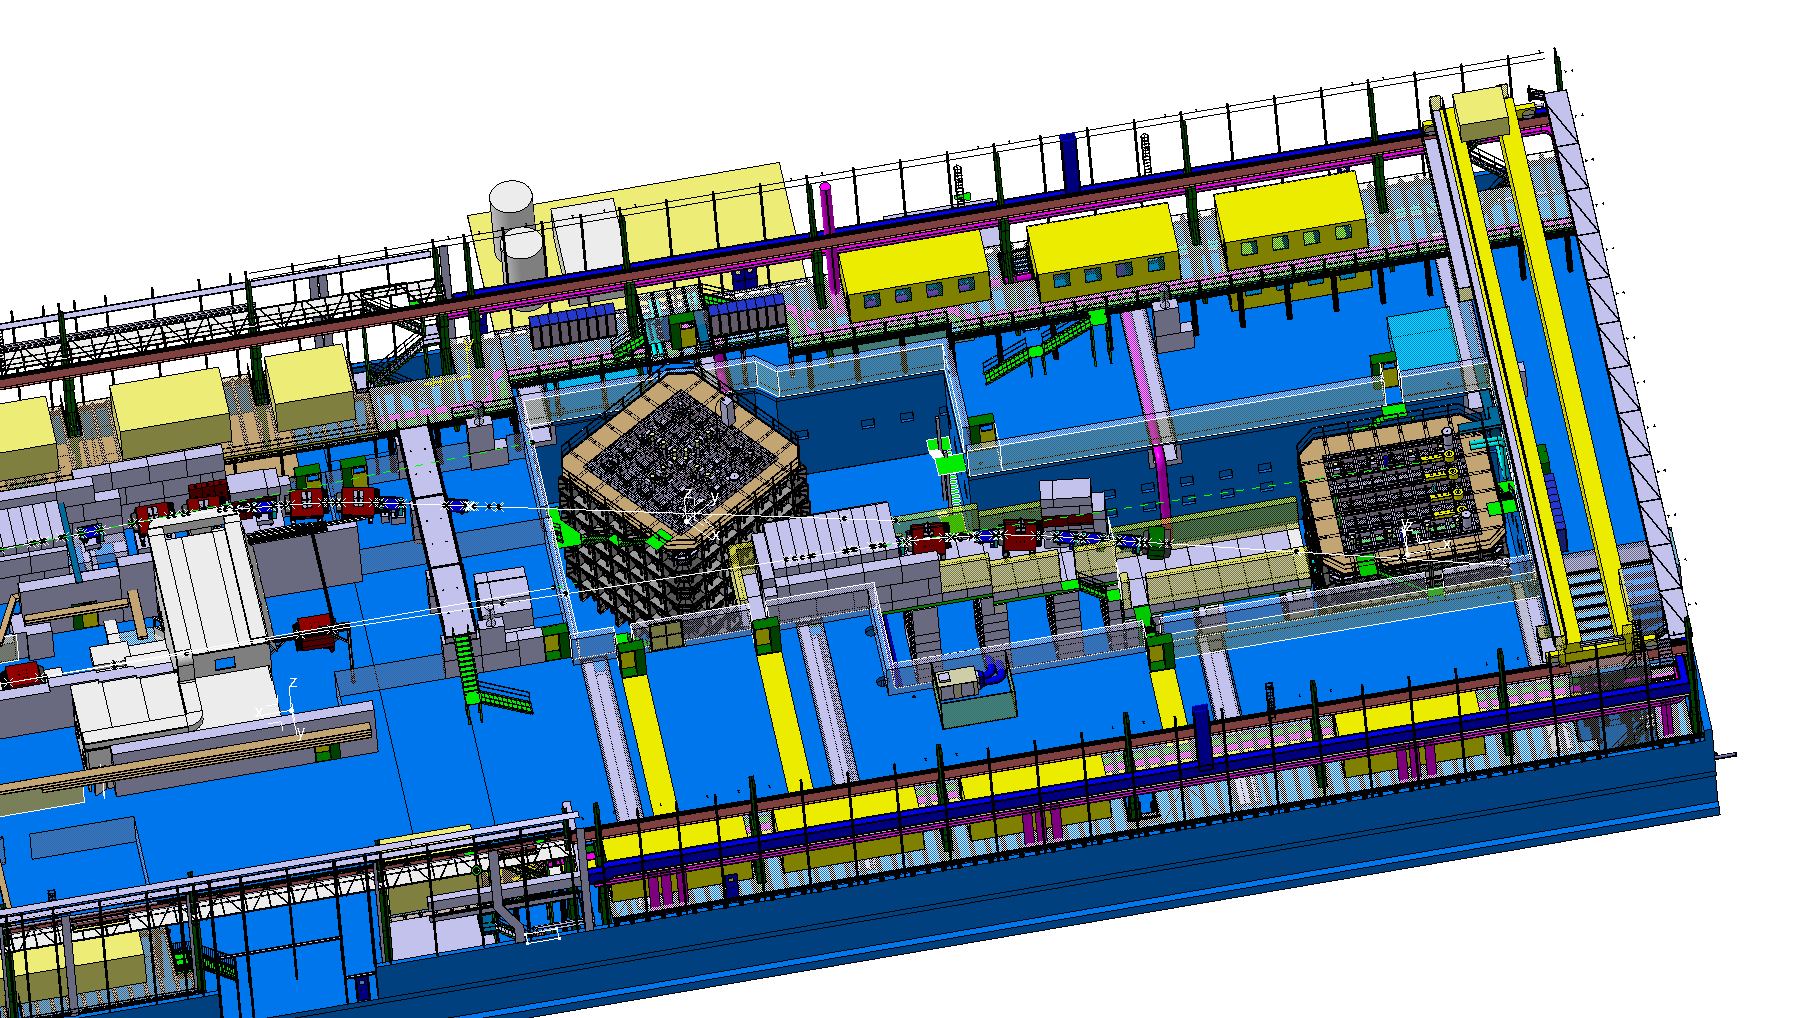
\includegraphics[width=1.0\textwidth]{figures/np02np04.png}

\caption{Please write your figure caption here}
\label{fig:np02np04}       % Give a unique label
\end{figure}

For two-column wide figures use syntax of figure~\ref{fig-2}
\begin{figure*}
\centering
% Use the relevant command for your figure-insertion program
% to insert the figure file. See example above.
% If not, use
\vspace*{5cm}       % Give the correct figure height in cm
\caption{Please write your figure caption here}
\label{fig-2}       % Give a unique label
\end{figure*}

For figure with sidecaption legend use syntax of figure
\begin{figure}
% Use the relevant command for your figure-insertion program
% to insert the figure file.
\centering
\sidecaption
%\includegraphics[width=5cm,clip]{tiger}
\centering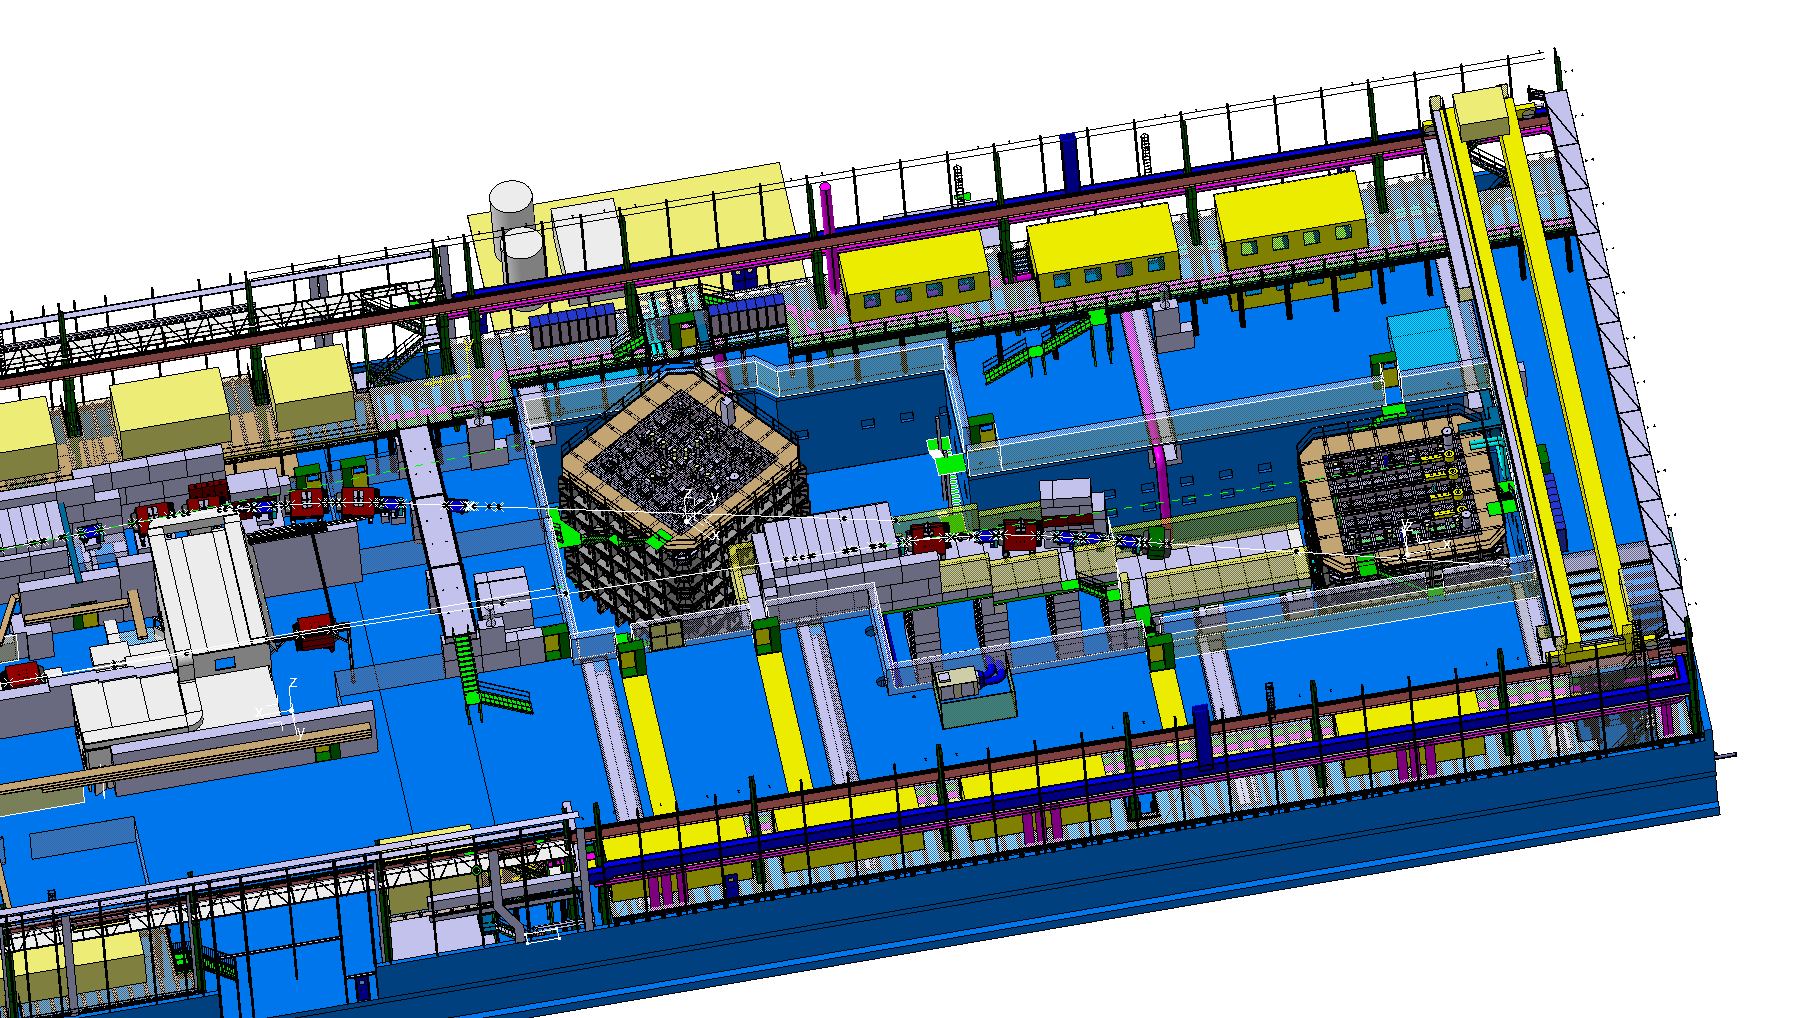
\includegraphics[width=1.0\textwidth]{figures/np02np04.png}
\caption{Please write your figure caption here}
\label{fig-3}       % Give a unique label
\end{figure}

For tables use syntax in table~\ref{tab-1}.
\begin{table}
\centering
\caption{Please write your table caption here}
\label{tab-1}       % Give a unique label
% For LaTeX tables you can use
\begin{tabular}{lll}
\hline
first & second & third  \\\hline
number & number & number \\
number & number & number \\\hline
\end{tabular}
% Or use
\vspace*{5cm}  % with the correct table height
\end{table}
%
% BibTeX or Biber users please use (the style is already called in the class, ensure that the "woc.bst" style is in your local directory)
% \bibliography{name or your bibliography database}
%
% Non-BibTeX users please use
%
\begin{thebibliography}{99}

\bibitem{cdrVol1}
R. Acciarri et al.
\emph{Long-Baseline Neutrino Facility (LBNF) and Deep Underground Neutrino Experiment (DUNE) Conceptual Design Report Volume 1: The LBNF and DUNE Projects}.\\ ~e-Print: arXiv:\textbf{1601.05471}
 %DUNE CDR Vol 1 -- The LBNF and DUNE Projects.~e-Print: arXiv:1601.05471
%\url{http://arxiv.org/abs/1601.05471}

\bibitem{cdrVol4}
R. Acciarri et al.
\emph{Long-Baseline Neutrino Facility (LBNF) and Deep Underground Neutrino Experiment (DUNE) Conceptual Design Report, Volume 4: The DUNE Detectors at LBNF}.\\~e-Print: arXiv:\textbf{1601.02984}
%\url{http://arxiv.org/abs/1601.02984}


\bibitem{uboone}
B. Jones et al.  \emph{The Status of the MicroBooNE Experiment.~J. Phys.: Conf. Series.} Vol.\textbf{408}. IOP Publishing, 2013,
doi:10.1088/1742-6596/408/1/012028

\bibitem{castoreos}
 L. Mascetti et al. \emph{Disk storage at CERN.~J. Phys.: Conf. Series.} Vol.\textbf{664}. IOP Publishing, 2015,
doi:10.1088/1742-6596/664/4/042035


\bibitem{sam}
R. A. Illingworth \emph{A data handling system for modern and future Fermilab experiments.~J. Phys.: Conf. Series.} Vol.\textbf{513}. IOP Publishing, 2014,
doi:10.1088/1742-6596/513/3/032045

\bibitem{fts}
A. Norman \emph{The Fermilab File Transfer System}.~e-Print: FNAL CD-DocDB-5412


\bibitem{xrootd}
L. Bauerdick et al. \emph{Using Xrootd to Federate Regional Storage.~J. Phys.: Conf. Series.} Vol.\textbf{396}. IOP Publishing, 2012,
doi:10.1088/1742-6596/396/4/042009

\bibitem{panda}
T. Maeno et al. \emph{Overview of ATLAS PanDA Workload Management.~J. Phys.: Conf. Series.} Vol.\textbf{331}. IOP Publishing, 2011,
doi:10.1088/1742-6596/331/7/072024



\bibitem{dirac}
A. Casajus et al.  \emph{DIRAC Pilot Framework and the DIRAC
Workload Management System.~J. Phys.: Conf. Series.} Vol.\textbf{219}. IOP Publishing, 2010,
doi:10.1088/1742-6596/219/6/062049

\bibitem{django}
N. George \emph{Mastering Django: Core. The Complete Guide to Django 1.8 LTS}~ GNW Independent Publishing, ISBN: 099461683X



\end{thebibliography}


\end{document}

% end of file template.tex

